% Documentclass options:
%    10pt, 11pt, 12pt  -- set type size
%    draft             -- single space, mark overfull hboxes on paper
%    final             -- double space, don't mark overfull hboxes on paper
%    oneside           -- format for one-sided printing
%    twoside           -- format for two-sided printing
% Defaults are 11pt,final,oneside.  Keep these, please.
\documentclass[11pt]{ucscthesisbs}
\bibliographystyle{apalike2}
\usepackage{natbib}
\usepackage{graphicx,epsf}% Include figure files


% The following declaration is for citations and bibliographies consistent with
% Astrophysical Journal specifications.  It may be left out or replaced with
% another bibliography/citation style.  See also the "\bibliographystyle"
% command later in this file.
%\usepackage{apj}

\usepackage{xcolor}
\usepackage{pagecolor}
\usepackage{lipsum}  

\pagecolor{darkgray}
\color{white}

% \pagecolor{white}
% \color{black}


\begin{document}

% Declarations for Front Matter

\title{Thermal Evolution of Uranus with Condensation-inhibited Convection}
\author{Robert Schroder}
\degreeyear{2020}
\degreemonth{November}
\degree{BACHELOR OF SCIENCE}
\field{ASTROPHYSICS}%
% Declare up to five committee members.  The text will be reproduced directly
% on the signature page.  Though the chair is a committee member, leave
% him/her out of the \committeemember declarations.  Make sure \numberofmembers
% agrees with the number of committee members declared INCLUDING the chair.
% If it is wrong, you will get extra or missing lines on the signature page.
%
\chair{Bruce Schumm}
\thesisadvisor{Christopher Mankovich}
\technicaladvisor{Jonathan Fortney}
\numberofmembers{3}




\campus{Santa Cruz}

\maketitle
\copyrightpage

\begin{frontmatter}

\begin{abstract}
This will be the last section written, once we have finished our analysis.
\end{abstract}

\tableofcontents
%
% The most recent (10/95) guidelines make absolutely no mention of the list
% of figures and list of tables.  Are they necessary?  If not, comment the
% next two lines out.
%
\listoffigures
\listoftables

\begin{dedication}
\null\vfil
{\large
\begin{center}
To Who,\\\vspace{12pt}
the owl
\end{center}}
\vfil\null
\end{dedication}

\begin{acknowledgements}
I'd like to thank my attorney, Bob Loblaw
\end{acknowledgements}


\end{frontmatter}

%\part{First Part}

\chapter{Introduction}
Observations of Uranus show a planet that appears to be in thermal equilibrium with the Sun. Observation has also shown that Uranus is cooler than its more distant neighbor, Neptune. Meanwhile, thermal evolution models for Uranus have not matched observation, instead predicting a warmer effective temperature during the current epoch\citep{fortney_2011}, \citep{podolak_1991}, \citep{hubbard_1995}, \citep{scheibe_2019} [There are other papers by Nettelmann 2013, Linder 2019 that I haven't looked at yet]. 

There have been various attempts to model the underluminous Uranus. [how much should i go into work done with different EOS's?] The formation of stable layers, trapping internal energy in the the interior of Uranus and Neptune was proposed by \citep{podolak_1991}. Work on the formation of stable condensation zones, inhibiting convection, have been investigated by \citep{friedson_2017}, \citep{leconte_2017}, and \citep{guillot_1995}. 


\chapter{Methodology}

[List out the equations of state that we are using, and what model atmosphere]



\begin{figure}[ht!]
 \centerline{
  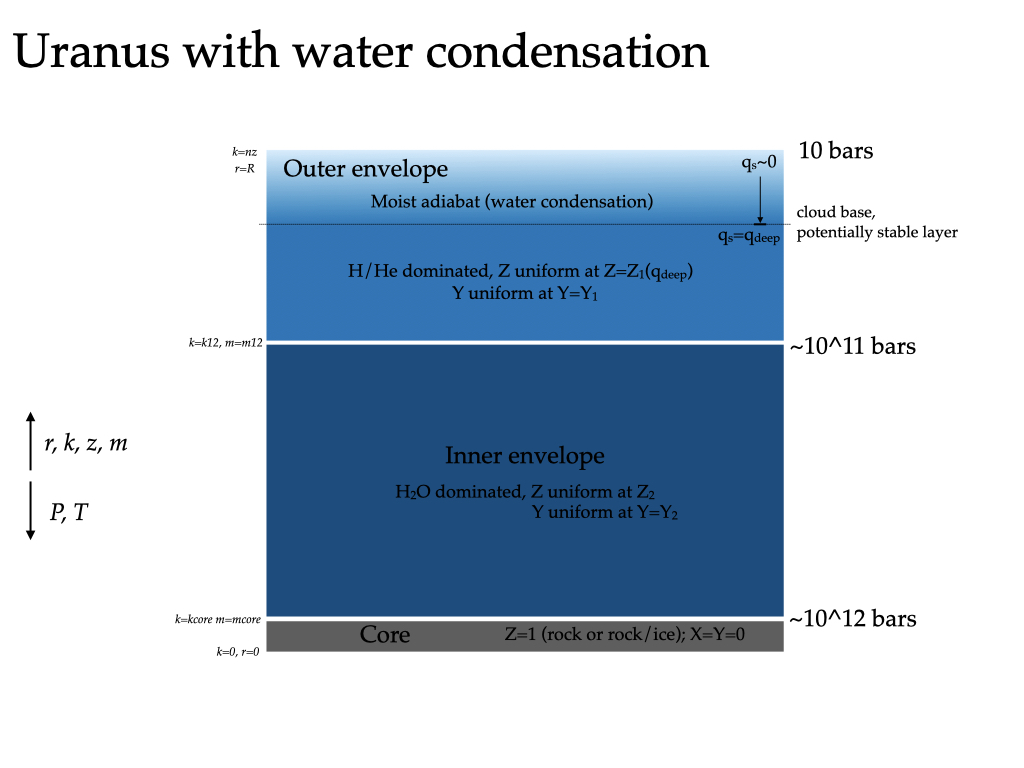
\includegraphics[width=7.0in]{figures/uranus_with_wcz_structure.001.jpeg}
 }
\caption[Interior Structure]
{Interior structure of Uranus with moist adiabatic layer}
\label{fig:uranus}
\end{figure}



\chapter{Results}

\section{Condensation-inhibited Convection}

\begin{figure}[ht!]
 \centerline{
  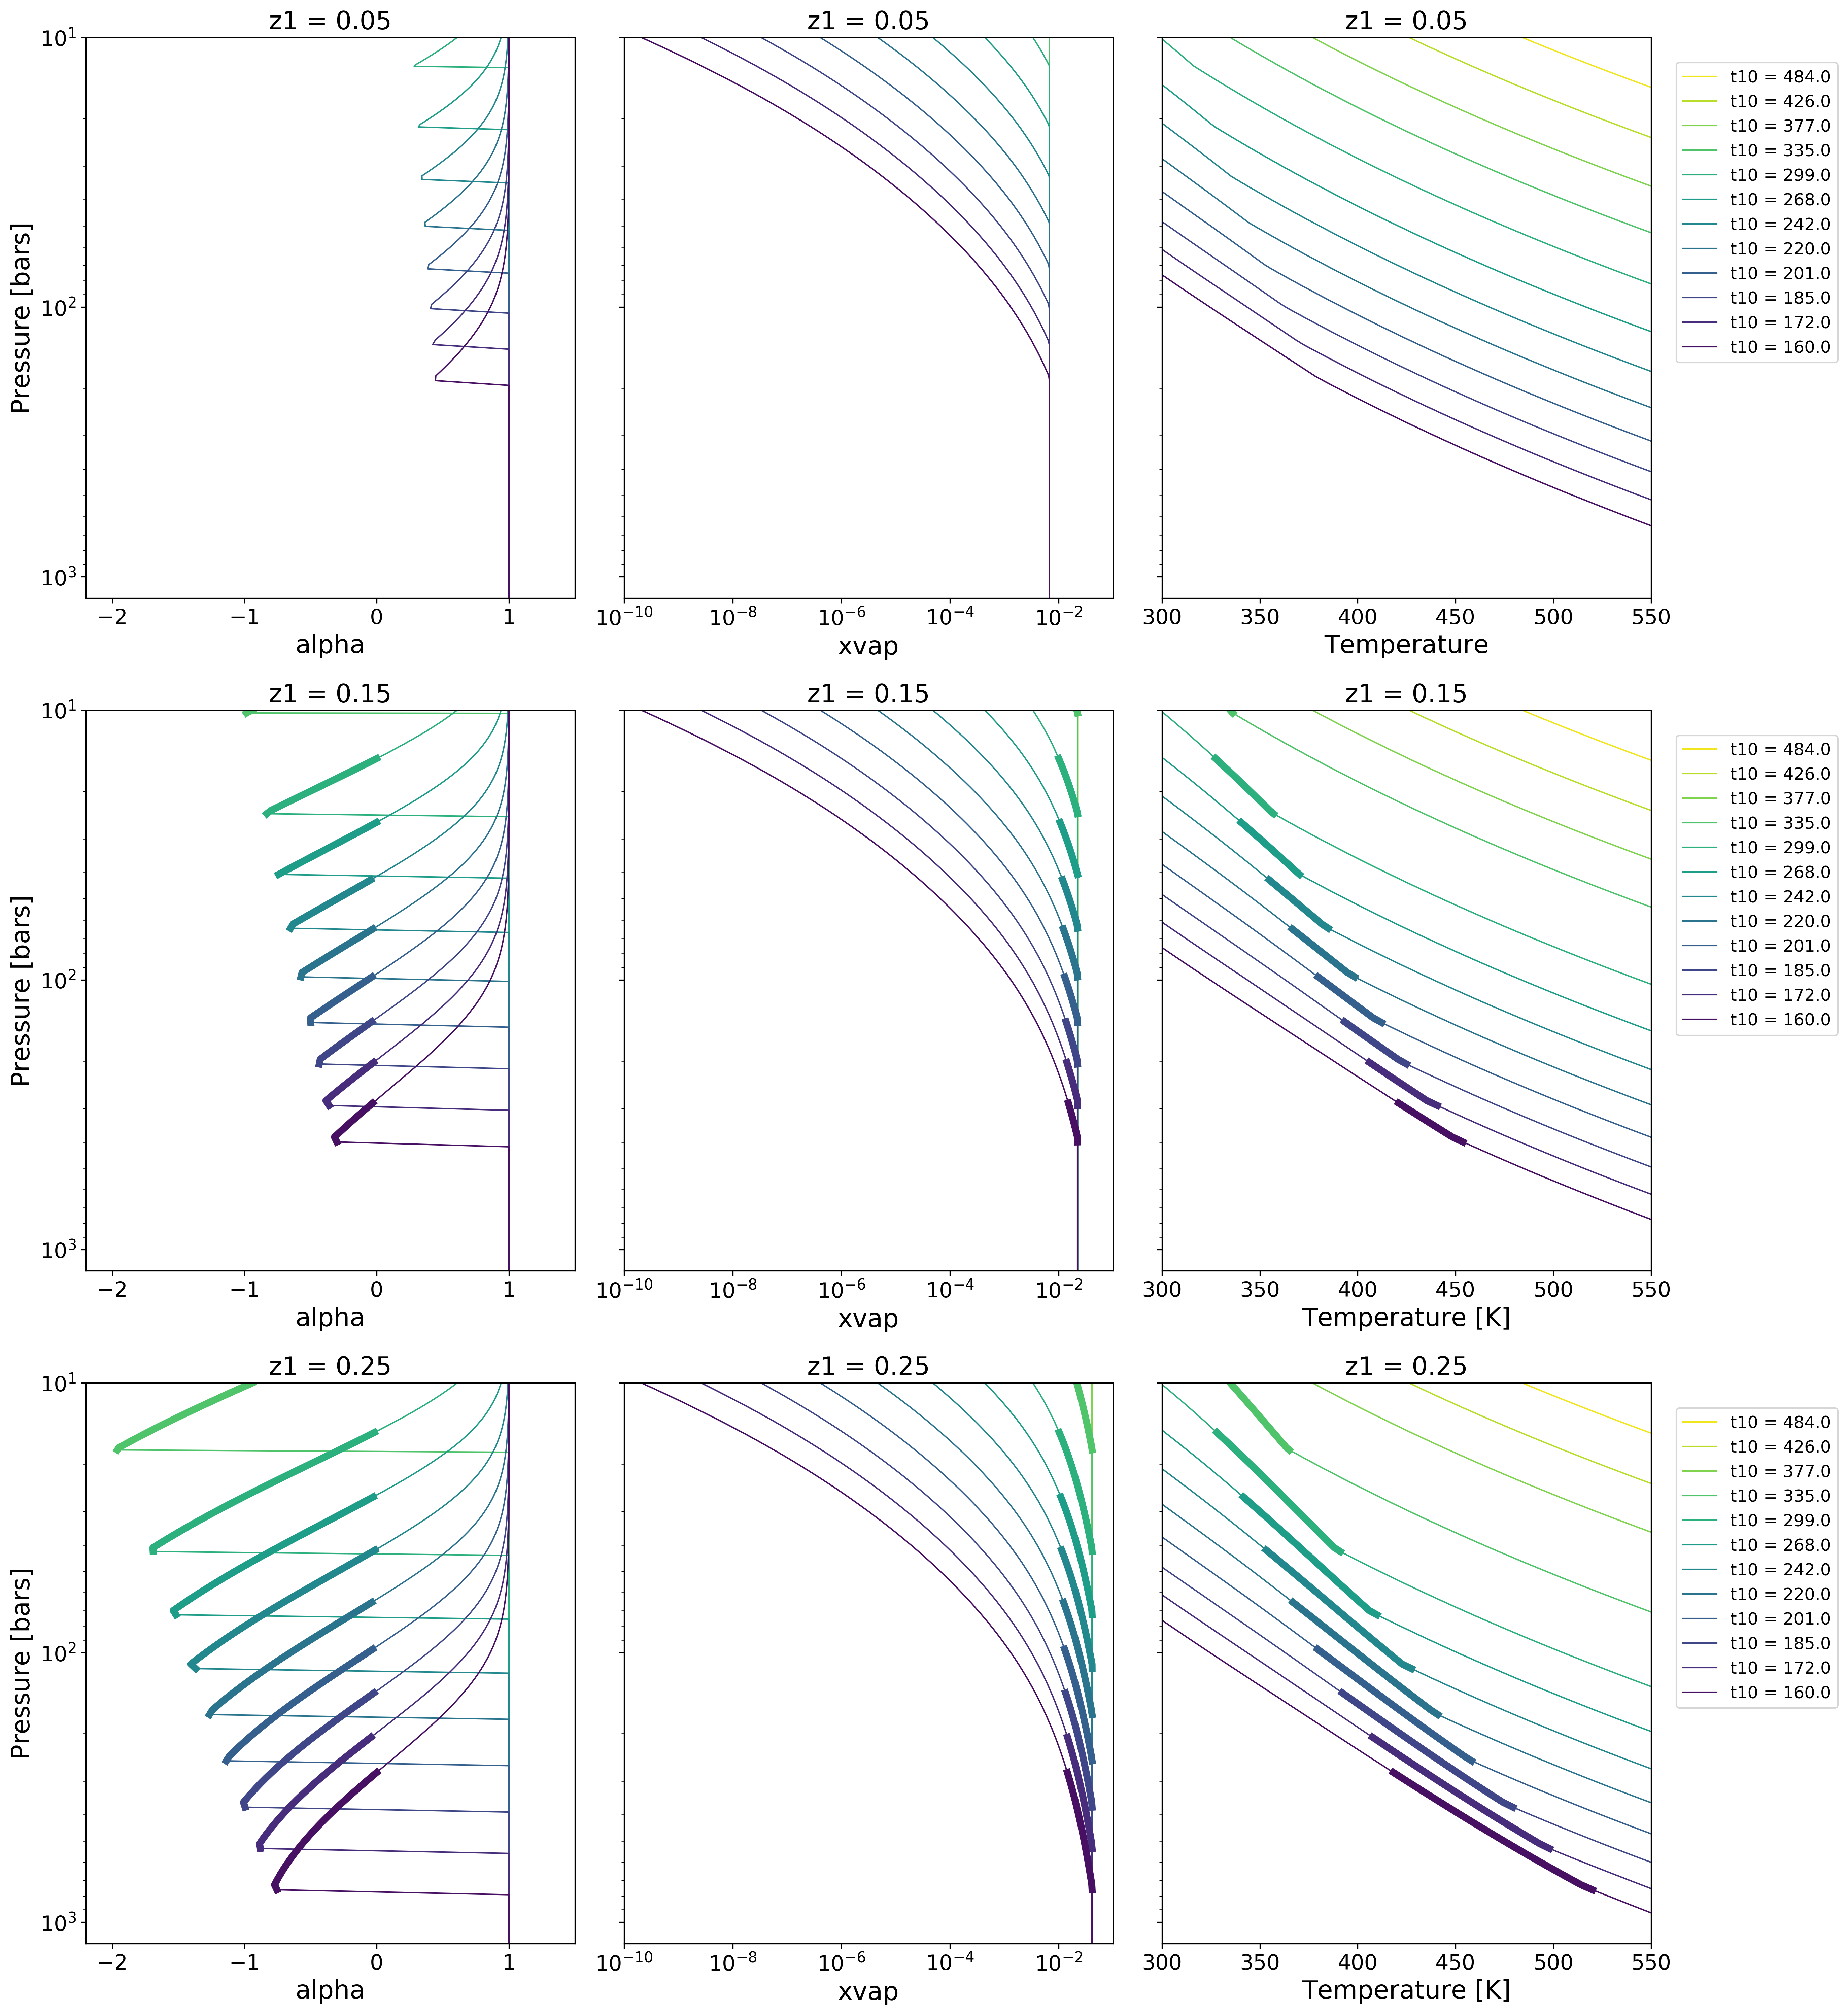
\includegraphics[width=7.0in]{figures/convection_inhibited_2.png}
 }
\caption[Inhibition of convection on Uranus]
{Need to add text here}
\label{fig:uranus}
\end{figure}

\section{Formation of Radiative Layer}

\begin{figure}[ht!]
 \centerline{
  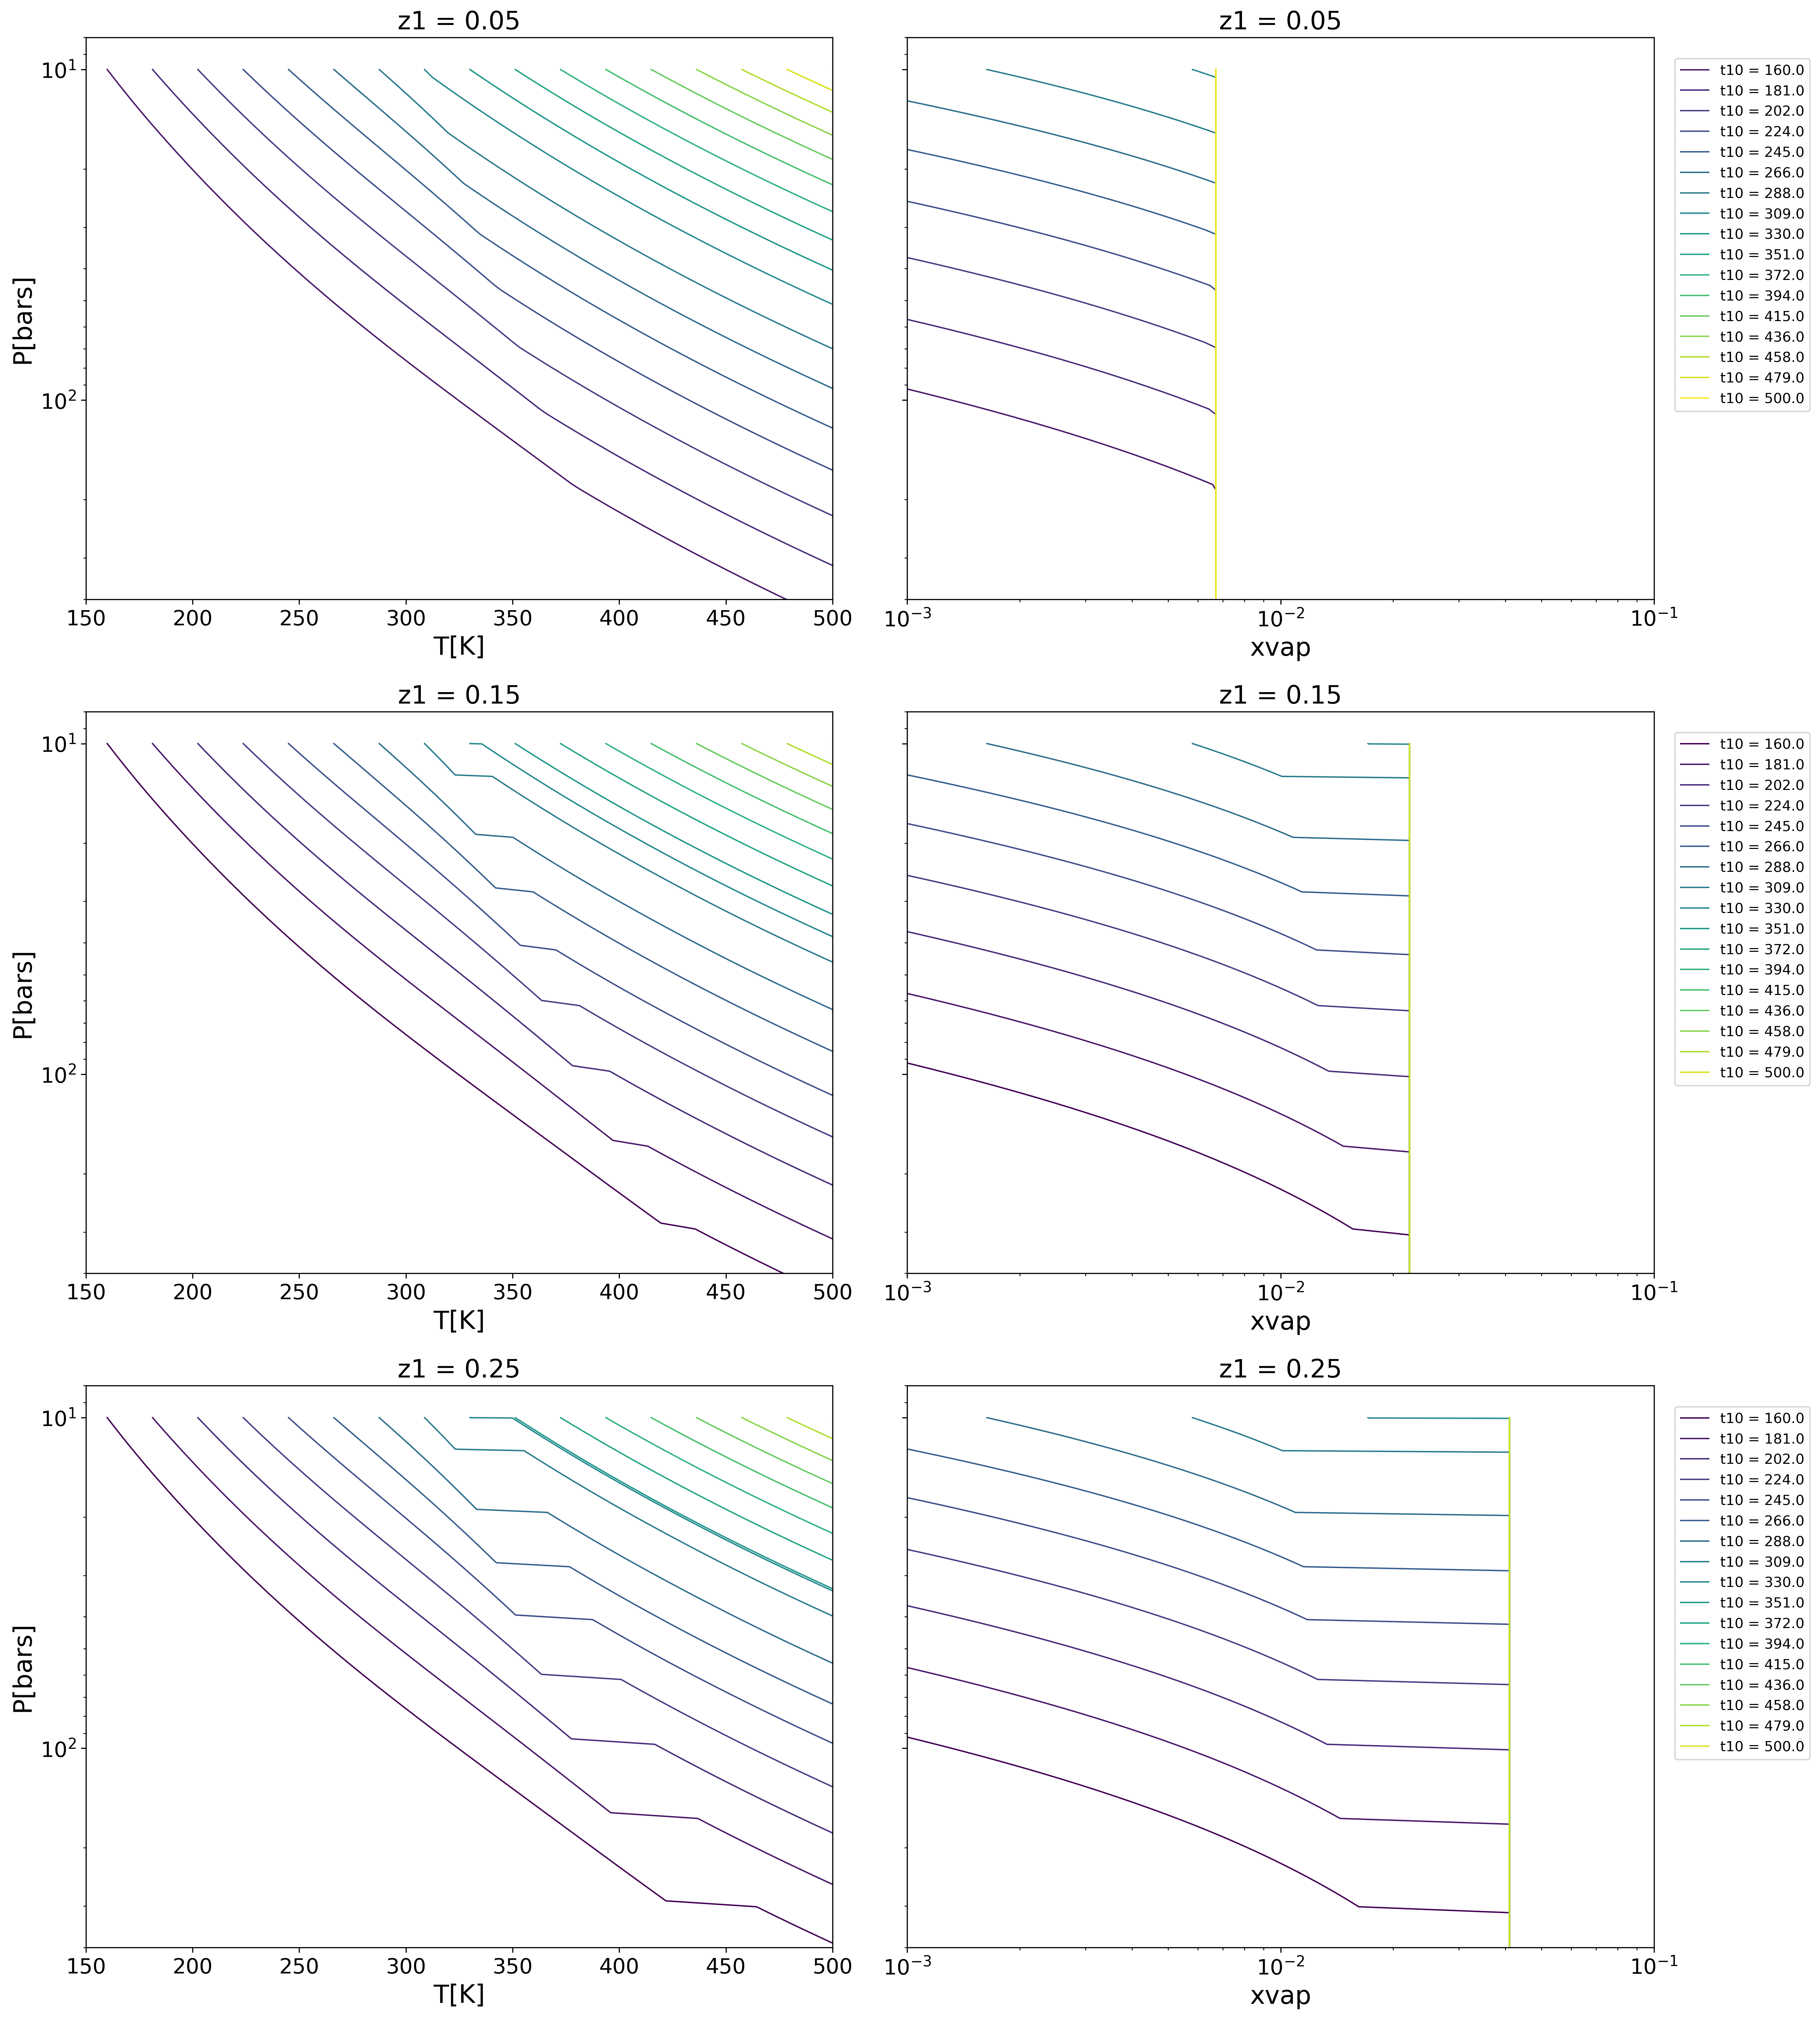
\includegraphics[width=7.0in]{figures/static_radiative_layer_plots_without_grid_points.png}
 }
\caption[Inhibition of convection on Neptune]
{Need to add description here }
\label{fig:neptune}
\end{figure}


\section{Thermal Evolution}




\chapter{Discussion and Conclusions}





\appendix
\chapter{Some Ancillary Stuff}


\bibliography{wcz_bib}


\end{document}
